%%%%%%%%%%%%%%%%%%%%
%%%%%%%%%%%%%%%%%%%%
\subsection{Examples}



\begin{table}[htbp!]
\begin{center}%
\caption{Examples of quantum states}
\label{TTtab:1}
\vspace{.2cm}
\begin{tabular}{|l|}
\hline
\textbf{\textit{Vacuum} state}  \\
$\bullet$ $\rho_{0,0}=1$ rest zero,\\
$\bullet$ $p_\rho(x|\phi)=e^{-x^2}/\sqrt{\pi}$. \\
%
\hline
\textbf{Single photon state}\\
$\bullet$ $\rho_{1,1}=1$ rest zero,\\
$\bullet$ $p_\rho(x|\phi)=2x^2e^{-x^2}/\sqrt{\pi}.$\\
%
\hline
\textbf{\textit{Coherent-$q_0$} state }$q_0\in\mathbb{R}$ \\
$\bullet$ $\rho_{j,k}=e^{-|q_0|^2}(q_0/\sqrt{2})^{j+k}/\sqrt{j!k!}$,\\
$\bullet$ $p_\rho(x|\phi)=\exp(-(x-q_0\cos(\phi))^2)/\sqrt{\pi}.$\\
%
\hline       
%\textbf{\textit{Squeezed state}}  $M\in\mathbb{R}_+$, $\xi\in\mathbb{R}$ \\
%$\bullet$ $\rho_{j,k}=C(M,\xi)(\frac 12
%\tanh(\xi))^{k+j}H_j(\delta)H_k(\delta)/\sqrt{j!k!}$,\\
%$\bullet$
%$p_\rho(x|\phi)=\exp\left[\left(\sin^2(\phi)(xe^{-2\xi}\cos(\phi)-(x\cos(\phi)-
%\alpha)e^{2\xi})^2\right)/\left(e^{2\xi}\sin^2(\phi)+e^{-2\xi}
%\cos^2(\phi)\right) \right.$\\
%$\quad$ $\quad$ $\quad$ $\quad$ $\times\left.-e^{-2\xi}(x\cos(\phi)-
%\alpha)^2-e^{2\xi}x^2\sin^2(\phi)
%\right]/\sqrt{\pi(e^{2\xi}\sin^2(\phi)+e^{-2\xi}\cos^2(\phi))}.$ \\
%
%\hline        
\textbf{\textit{Thermal state}} $\beta>0$\\
$\bullet$ $\rho_{j,k}=\delta^j_k(1-e^{-\beta})e^{-\beta k}$,\\
$\bullet$ $p_\rho(x|\phi)=\sqrt{\tanh(\beta/2)/\pi}\exp(-x^2\tanh(\beta/2)).$\\
%
\hline
\textbf{\textit{Schr\"{o}dinger cat}} $q_0>0$ \\
$\bullet$
$\rho_{j,k}=2(q_0/\sqrt{2})^{j+k}/\left(\sqrt{j!k!}
(\exp(q_0^2/2)+\exp(-q_0^2/2))\right)$, for $j$ and $k$ even, rest zero,\\
$\bullet$ $p_\rho(x|\phi)=\left(\exp(-(x-q_0\cos(\phi))^2)+\exp(-(x+q_0
\cos(\phi))^2)\right.$\\
$ \quad$ $ \quad$ $ \quad$ $ \quad$
$\left.+2\cos(2q_0x\sin(\phi))\exp(-x^2-q_0^2\cos^2(\phi))\right)%$%\\
 %$ \quad$ $ \quad$ $ \quad$ $ \quad$  
 /\left(2\sqrt{\pi}(1+\exp(-q_0^2))\right).$\\
 \hline
\end{tabular}
\end{center}
\end{table}

 %A state is called pure if it cannot be represented as a mixture (convex combination) of other states, i.e., if it is an extreme point of the convex set of states. This is equivalent to the density matrix being a one dimensional projector, i.e., of the form $\rho=\textbf{P}_{\psi}$ for some unit vector $\psi$. In this case the formula for the expectation value of an operator $A$ in the state simplifies as $tr(A\rho)=E_\rho[A]$. Equivalently, a state $\rho$ is pure if $\text{Tr}(\rho^2)=1$. All other states are called mixed states.\\
We present in Table~\ref{TTtab:1} examples of pure quantum states, which can be
created at this moment in laboratory and belong to the class $\mathcal{R}(C,B,r)$ with $r=2$.   Table~\ref{TTtab:1} gives also their explicit density matrix coefficients $\rho_{j,k}$ and probability densities $p_\rho(x|\phi)$.\\
Among the pure states we consider the \textit{vacuum} state, which is the pure state of zero photons. Note that the \textit{vacuum} state would
provide a random variable of Gaussian probability density $p_\rho(x|\phi)$ via the ideal measurement of QHT (see Section~\ref{QHT}). That explains the gaussian nature of the noise in the effective result of the QHT measurement. \\
The \textit{single photon} state, which is the pure state of one photon. We consider also the \textit{coherent-$q_0$} state, which characterizes the laser pulse with the number of photons  Poisson distributed with an average of $M$ photons.
% The \textit{Squeezed} states (see e.g. \cite{Breitenbach&Schiller&Mlynek}) have Gaussian Wigner functions whose variances in the two directions have a fixed product. The parameters $M$ and $\xi$ are such that $M\geq \sinh^2(\xi)$,$C(M,\xi)$ is a normalization constant, $\alpha=\frac{(M-\sinh^2(\xi))^{1/2}}{\cosh(\xi)-\sinh(\xi)}$, and $\delta=\left(\frac{\alpha}{\sinh(2\xi)}\right)^{1/2}$.
Remark that the well-known \textit{Schr\"{o}dinger cat} state is described by a linear
superposition of two \textit{coherent} vectors (see e.g. \cite{Our}).



%%%%%%%%%%%%%%%%%%%%%%
\subsection{Pattern functions $f^\eta_{j,k}$}
\label{TTsimu.pattern.function}
%%%%%%%%%%%%%%%%%%%%%%

Since there is no closed-form expression for the pattern functions $f^\eta_{j,k}$, we evaluate them numerically on a 1-D regular grid of $Q=4096$ points. We use expressions~\eqref{Rpattern} and~\eqref{eq:patterneta} to evaluate $\tilde f_{j,k}$ and $\tilde f_{j,k}^\eta$  on the 1-D frequency grid of $Q$ discretized $t$ points. The adapted pattern functions $f_{j,k}^\eta$ are computed on the 1-D spacial grid of $Q$ discretized $x$ points by applying to $\tilde f_{j,k}^\eta$ the inverse Fast Fourier Transform (FFT) in $O(Q \log(Q))$ operations. Figure~\ref{fig:example-pattern} shows a few examples of pattern functions. 


\begin{figure}[!h]
\begin{center}
\begin{tabular}{@{}c@{\hspace{1mm}}c@{}}
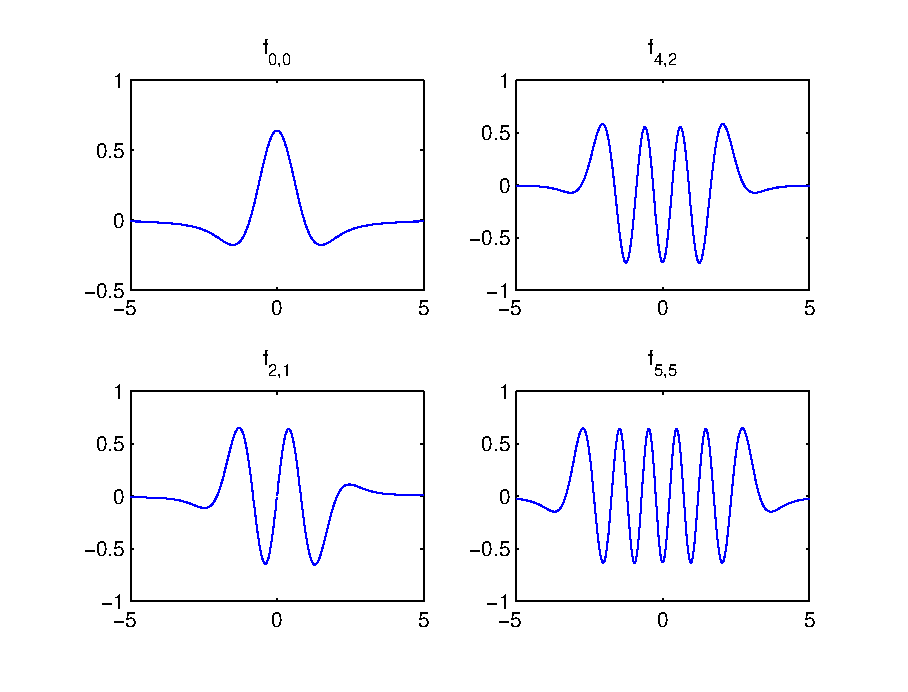
\includegraphics[width=.49\linewidth]{pattern}&
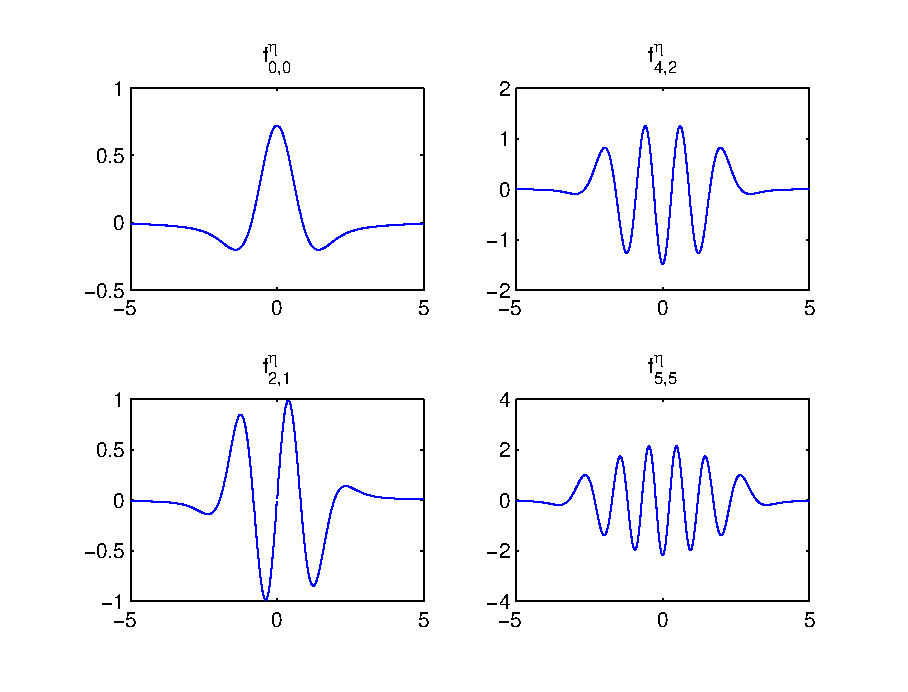
\includegraphics[width=.49\linewidth]{patterneta}\\
\end{tabular}
\caption{ % 
	Examples of pattern functions $f_{j,k}$ (left) and adapted pattern functions $f_{j,k}^\eta$ (right).
}
\label{fig:example-pattern}
\end{center}
\end{figure}



%%%%%%%%%%%%%%%%%%%%%%%
\subsection{Implementation of our procedure}
\label{TTimplementation.Mn}
%%%%%%%%%%%%%%%%%%%%%%%


The deconvolved estimator $\hat{\rho}^\eta_{j,k}$ defined in~\eqref{estrhojk} is computed by evaluating $ G_{j,k}(x,\phi) = f^\eta_{j,k}(x) e^{-i(j-k)\phi}$ at point $x$ using a cubic spline interpolation of the values of $f^\eta_{j,k}$ on the discrete grid of $Q$ points.

In the following section, we evaluate the performance of the threshold estimator $\tilde{\rho}^{\eta}_{j,k}$. We perform this evaluation by creating noisy samples $Y_\ell$ as defined in~\eqref{noisy.data}. The initial samples $X_\ell$ are drawn from the distribution $p_\rho(x | \phi)$ (see Table~\ref{TTtab:1}) using the rejection method. 

The value of $N=N(n)$ is set following~\eqref{Ncorr1}. We use $r_0=2$ and $B_0=1/2$ for all the numerical experiments.

A toolbox that implements this procedure and reproduces all the figures of this article is available online\footnote{\url{http://www.ceremade.dauphine.fr/~peyre/codes/}}.

%%%%%%%%%%%%%%%%%%%%%%%%%%%%%%%
\subsection{Studies of the performance of our test procedure }
\label{TTperformanceOmega}
%%%%%%%%%%%%%%%%%%%%%%%%%%%%%%%



\newcommand{\myfiga}[1]{\includegraphics[width=.32\linewidth]{#1/#1-rho}}
\newcommand{\myfig}[3]{\includegraphics[width=.32\linewidth]{#1/b0-#2/#1-n#3}}
% Change this value to select a different B0=\Bvalue/10 value.
\newcommand{\Bvalue}{5}
\newcommand{\vertText}[1]{ \rotatebox{90}{\mbox{\hspace{1cm} #1}}   }
\begin{figure}[!h]
\begin{center}
\begin{tabular}{@{}c@{\hspace{1mm}}c@{\hspace{1mm}}c@{\hspace{1mm}}c@{}}
\vertText{$\rho$} & \myfiga{coherent}   				&  \myfiga{shrodinger-cat}				&   \myfiga{thermal}					\\
\vertText{$n=10^4$} & \myfig{coherent}{\Bvalue}{10k}	&   \myfig{shrodinger-cat}{\Bvalue}{10k}	&   \myfig{thermal}{\Bvalue}{10k}			\\
\vertText{$n=10^5$} & \myfig{coherent}{\Bvalue}{100k}	&   \myfig{shrodinger-cat}{\Bvalue}{100k}	&   \myfig{thermal}{\Bvalue}{100k}			\\
\vertText{$n=10^6$} & \myfig{coherent}{\Bvalue}{1000k}	&   \myfig{shrodinger-cat}{\Bvalue}{1000k}	&   \myfig{thermal}{\Bvalue}{1000k}	\\
\vertText{$n=10^8$} & \myfig{coherent}{\Bvalue}{100000k}	&   \myfig{shrodinger-cat}{\Bvalue}{100000k}	&   \myfig{thermal}{\Bvalue}{100000k}	\\
    & Coherent $q_0=3$ &
Schr\"{o}dinger cat $q_0=3$ &
Thermal $\beta=1/4$
\end{tabular}
\caption{First row: $\rho$.
  Following rows: estimated $\tilde \rho^\eta$ for $B_0=0.\Bvalue{}$, $\eta=0.9$, $\varepsilon=1$ and $n$ respectively equal to 
  $10^4$ (row \#2), 
  $10^5$ (row \#3), 
  $10^6$ (row \#4), 
  $10^8$ (row \#5). }
\label{fig:examples}
\end{center}
\end{figure}

Figure~\ref{fig:examples} shows graphically the result of our estimator for three different pure quantum states, for several values of $n$. To further evaluate quantitatively the performance of the method, we estimate numerically the (relative) root mean square error (RMSE) 
\begin{equation*}
	\text{RMSE}(n) = \frac{ \| \tilde \rho^\eta - \rho \| }{�\| \rho \| }
\end{equation*}
of our soft thresholding estimator. More precisely, Figure~\ref{fig:RMSE} shows the evolution with $n$ of the expected value of the RMSE. This expected value is evaluated by an empirical mean with Monte Carlo simulation using 50 samplings for each value of $n$. To evaluate the deviation with respect with this mean, we also display the confidence interval at $\pm 3$ times the standard deviation of the RMSE. 

The threshold values $t_{j,k}$ that are used in~\eqref{rho-seuil} to define our estimator are somehow conservative. In practice, smaller values offer better decay of the RMSE. Figure~\eqref{fig:RMSE} display in dashed red (reap. dashed green) the decay of the RMSE obtained using thresholds $0.8 t_{j,k}$ (resp. $0.5 t_{j,k}$). We found on these three examples and for $\eta=0.9$ that using $0.5 t_{j,k}$ gives consistently the lowest RMSE among other choices of thresholds proportional to the $t_{j,k}$ values.

\begin{figure}[!h]
\begin{center}
\begin{tabular}{@{}c@{\hspace{1mm}}c@{}}
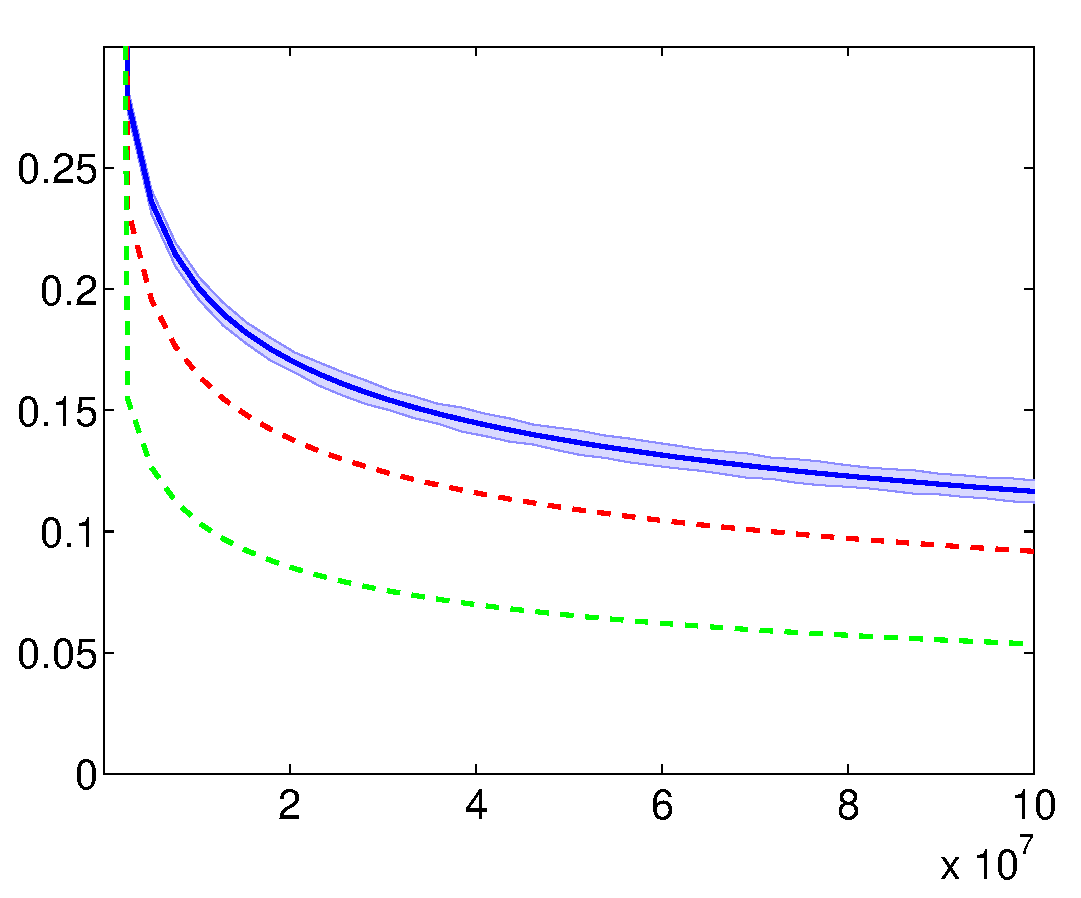
\includegraphics[width=.45\linewidth]{results-rmse/coherent-eta9-rmse}&
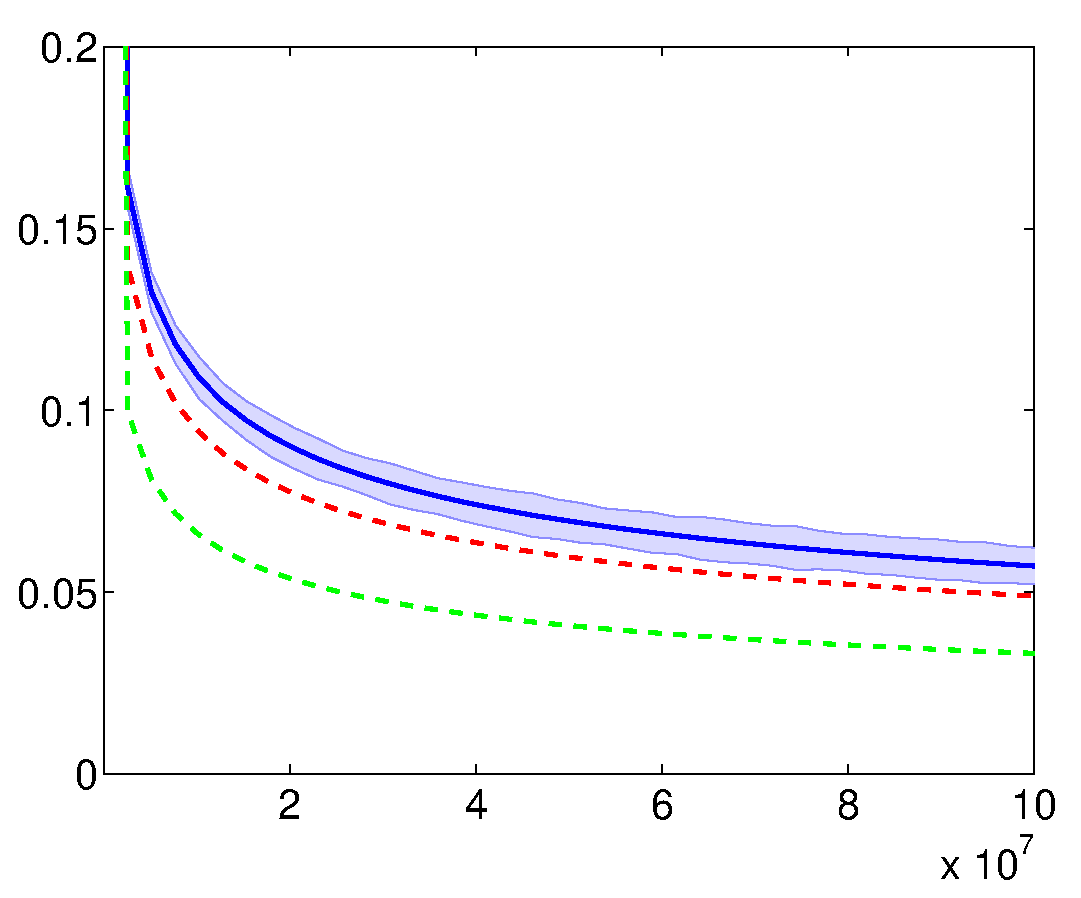
\includegraphics[width=.45\linewidth]{results-rmse/shrodinger-cat-eta9-rmse}\\
Coherent $q_0=3$ &
Schr\"{o}dinger cat $q_0=3$ \\
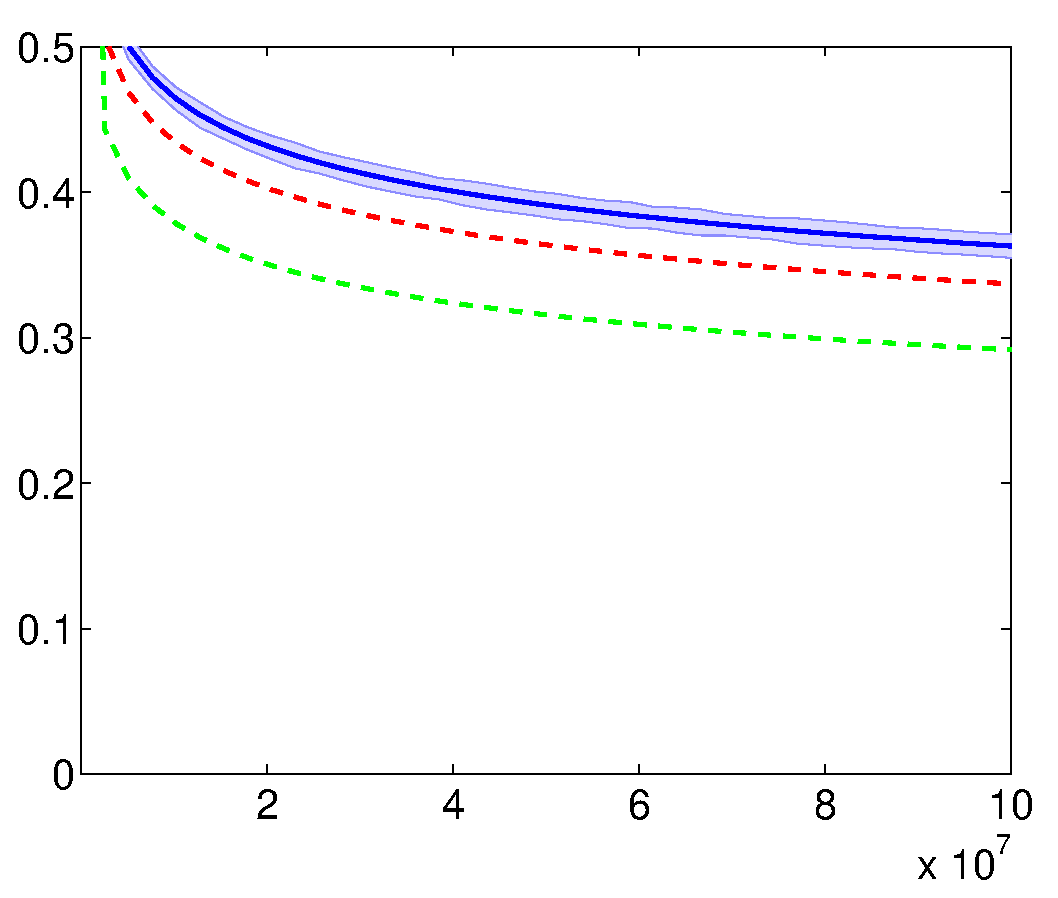
\includegraphics[width=.45\linewidth]{results-rmse/thermal-10-eta9-rmse}& 
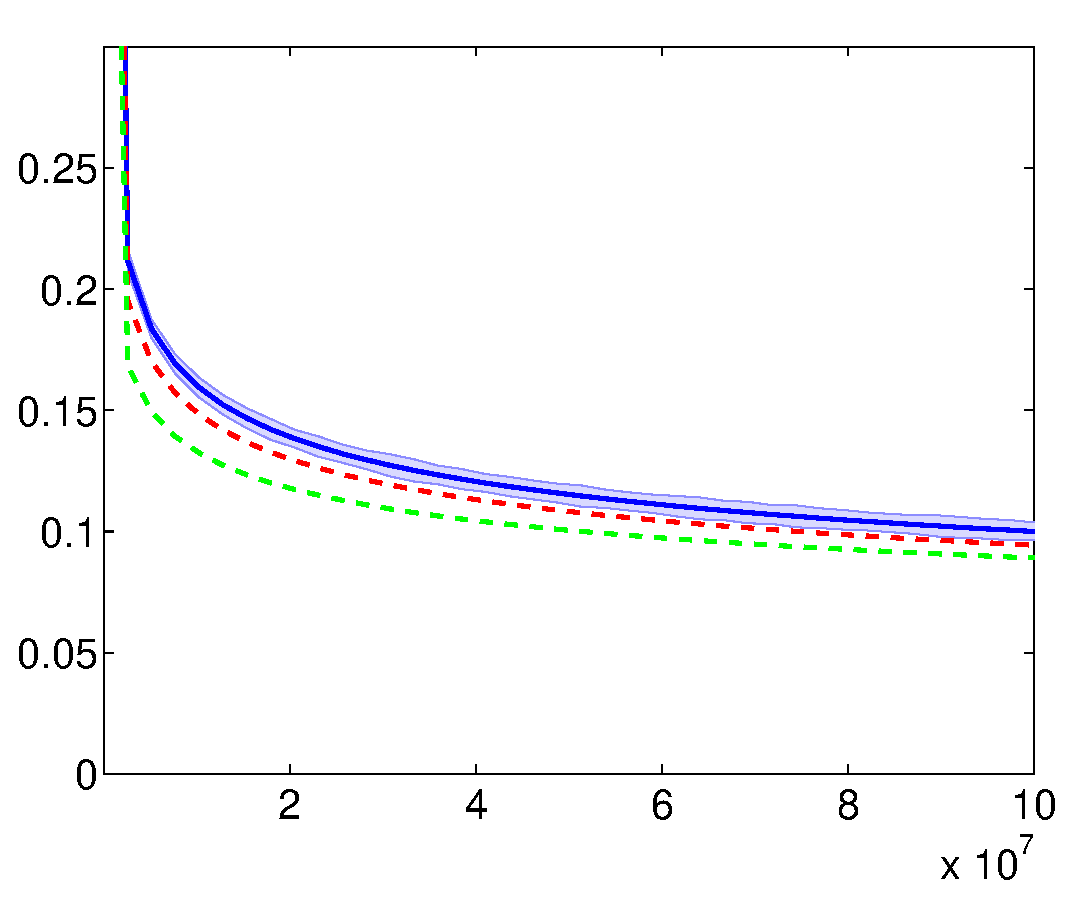
\includegraphics[width=.45\linewidth]{results-rmse/thermal-25-eta9-rmse} \\
Thermal $\beta=1/10$  & Thermal $\beta=1/4$
\end{tabular}
\caption{ % 
	Blue curve: Evolution of $\mathbb{E}( \text{RMSE}(n) )$ as a function of $n$ for $\eta=0.9$, $\varepsilon=1$.
	The blue shaded area represent the confidence interval 
	at $\pm 3$ times the standard deviation of RMSE$(n)$.
	Red (reps. green) curve: evolution of $\mathbb{E}( \text{RMSE}(n) )$ obtained when replacing the threshold $t_{j,k}$ by $0.8 t_{j,k}$ (resp. $0.5 t_{j,k}$) in the estimator in~\eqref{rho-seuil}.
}
\label{fig:RMSE}
\end{center}
\end{figure}

We found numerically that the decay of the RMSE with $n$ almost perfectly fits a power-law, which (up to logarithmic factor) is in accordance with the upper-bounds of Corollary~\ref{coro1}. Following this Corollary in the setting $\eta\in(\frac{1}{2},1)$ and $ r=2$,  we fit a power law of the form 
\begin{equation*}
	\mathbb{E}(\text{RMSE}(n)) \approx n^{ -\frac{\tilde B}{2 ( 4 \gamma+\tilde B)} }.
\end{equation*}
We perform a linear regression in a log-log domain to estimate $\tilde B$. 
Table~\ref{tab:B} reports the estimated value of $\tilde B$ we found using this procedure. 

\begin{table}[!h]
\caption{Estimated values of $\tilde B$ when using $\eta=0.9$, $\varepsilon=1$ and $N=30$.}
\label{tab:B}
\begin{center}
\begin{tabular}{|c|c|c|c|}
\hline 
Coherent $q_0=3$ &
Schr\"{o}dinger cat $q_0=3$ &
Thermal $\beta=1/10$ & 
Thermal $\beta=1/4$ \\ \hline
$\tilde B \approx 0.174$ &
$\tilde B \approx 0.227$ &
$\tilde B \approx 0.037$ & 
$\tilde B \approx 0.082$ \\\hline
\end{tabular}
\end{center}
\end{table}


